Jako první určíme proud \(I_d\), to uděláme dvěma způsoby, podle požadovaného \(SR\) a podle požadovaného \(GBW\) a vybereme ten větší.


Podle \(SR\)
\begin{center}
    \large
    \(
        I_d = SR \cdot C_L = 5 \cdot 10^{6} \cdot 2 \cdot 10^{-12} = 10 [\mu A]
    \)
\end{center}

Podle \(GBW\) 
\begin{center}
    \large
    \(
        I_d = GBW \cdot U_{OV} \cdot \pi C_L = 6M \cdot 0.2 \cdot \pi \cdot 2p = 7.54 [\mu A]
    \)
\end{center}

Proud teď bude \(I_d = 10 [\mu A]\) 

Dále můžeme určit rozměry tranzistoru, k čemuž budeme muset zvolit napětí \(U_{OV}\), která volím s ohledem na pracovní rozsah \(U_{OV} = 0.2 [V]\).
Délku tranzistoru \(L\) zvolím s ohledem na parametr \(\lambda\) \(L = 2 [\mu m]\).

\begin{center}
    \large
    \(
        W = L \cdot \frac{2 \cdot I_d}{KP \cdot U_{OV}^2} = 2\mu \cdot \frac{2 \cdot 10\mu}{50\mu 0.2^2} = 20 [\mu m]
    \)
\end{center}

Dále můžeme z Ohmova zákona určit zatěžovací rezistor \(R_D\) jako:

\begin{center}
    \Large
    \(
        R_D = \frac{U_{out}}{I_D} = \frac{0.9}{10\mu} = 90 [k\Omega] 
    \)
\end{center}

\vspace{10mm}
\begin{figure}[h!]
    \centering
    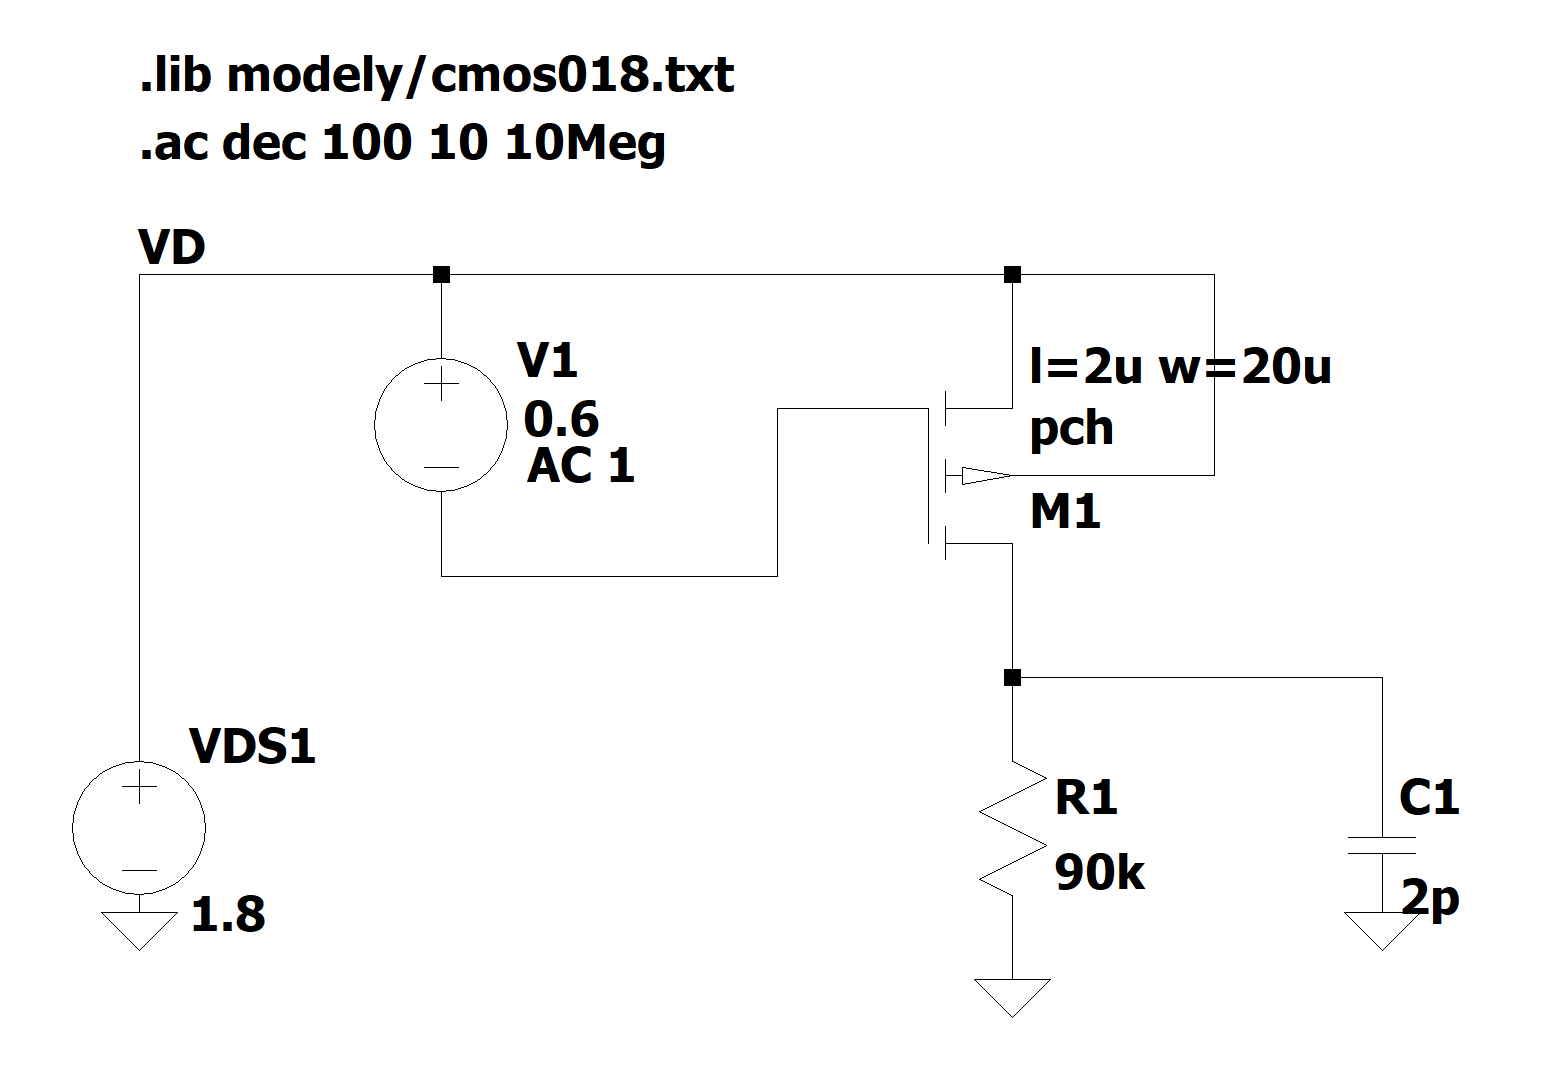
\includegraphics[width=0.6\textwidth]{text/img/Res-sch.png}
    \caption{\label{fig:res-sch} Schéma zesilovače}
\end{figure}

\vspace{10mm}
\begin{figure}[h!]
    \centering
    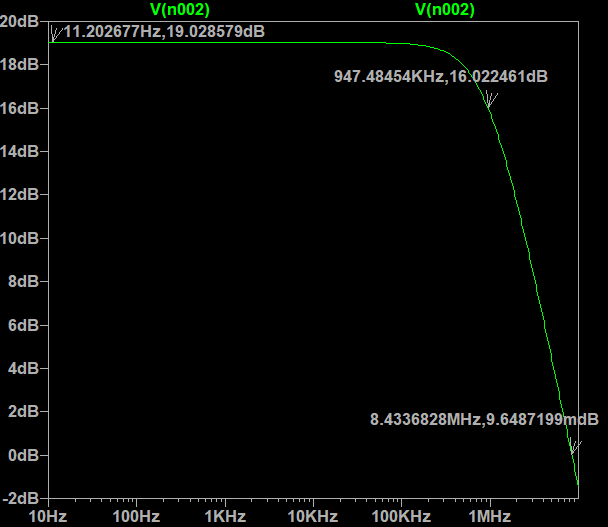
\includegraphics[width=0.8\textwidth]{text/img/Res-AC-graf.png}
    \caption{\label{fig:res-AC} {\bf .AC} analýza zesilovače}
\end{figure}
Zesílení mi vychází o necelý decibel menší než dle zadání, zkusil jsem tedy lehce zvětšit zatěžovací odpor na hodnotu \(R_1 = 102.48 [k\Omega]\) a obdržel jsem průběh \ref{fig:res-AC-102.48k}

\begin{figure}[h!]
    \centering
    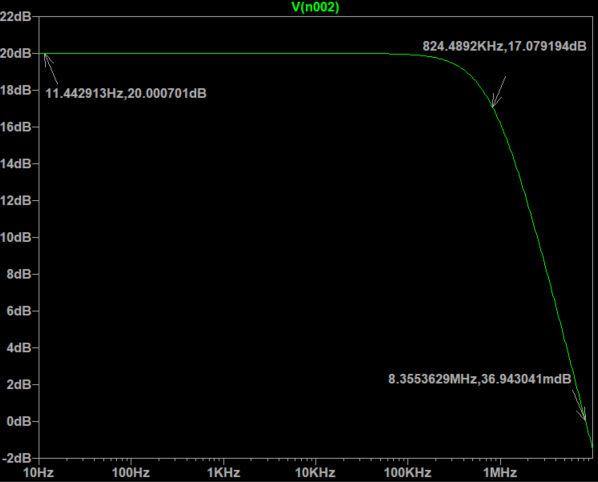
\includegraphics[width=0.8\textwidth]{text/img/Res-AC-graf-102.48k.png}
    \caption{\label{fig:res-AC-102.48k} {\bf .AC} analýza zesilovače se zvětšeným zatěžovacím odporem na \(R_1 = 102.48 [k\Omega]\)}
\end{figure}

\vspace{10mm}
\begin{figure}[h!]
    \centering
    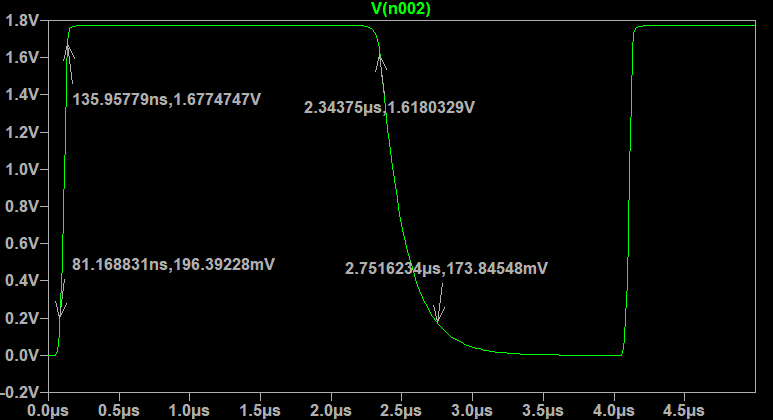
\includegraphics[width=0.9\textwidth]{text/img/Res-trans-graf.png}
    \caption{\label{fig:res-SR} {\bf .trans} analýza s vyznačenými body pro určení SR}
\end{figure}

Z průběhu \ref{fig:res-SR} určíme SR jako:
\begin{center}
    \Large
    \(
        SR_{rise} = \frac{\Delta U}{\Delta t} = \frac{U_2 - U_1}{t_2 - t_1} = \frac{1.677 - 0.196}{126n - 81n} = 32.9 [V/\mu s]
    \)

    \(
        SR_{fell} = \frac{\Delta U}{\Delta t} = \frac{U_1 - U_2}{t_2 - t_1} = \frac{1.618 - 0.174}{2752n - 2344n} = 3.5 [V/\mu s]
    \)
\end{center}

Sestupná hrana je pomalejší, než by dle zadání měla být, což je způsobeno předpokladem lineárního vybíjení kondenzátoru \(C_1\), zatím co je exponenciální, jak je vidět na průběhu \ref{fig:res-SR}

\(GBW\) je větší, než bylo požadováno, protože proud tranzistorem jsme stanovili vyšší, abychom splnili \(SR\).